\subsection{Bookkeeping}
A peer will upload to and download from other peers in the network.
The peer will want to increase his reputation and have a transaction transcribing his contribution.
The transaction contains the information about how much data was uploaded and downloaded between the peers
and their total upload and download amounts.

Every peer in Dispersy has a public and private key that can be used to identify them.
A block contains both public keys of the peers,
so it is possible to see to which peers the transaction belongs to.
Every block only contains one transaction.
An overview can be seen in Figure \ref{fig:block}

\begin{figure}
	\centerline{\includegraphics[scale=0.3]{design/figs/block.eps}}
	\caption{A block in MultiChain.}
	\label{fig:block}
\end{figure}

The transaction will be stored inside a single block.
The blocks are linked to previous blocks by adding the hashes of the previous blocks of both peers.
This creates a directed acyclic graph of blocks.
An overview of a chain of blocks is seen in Figure \ref{fig:transaction-chain}.
In this overview the chain of B is currently ignored.

\begin{figure}
	\centerline{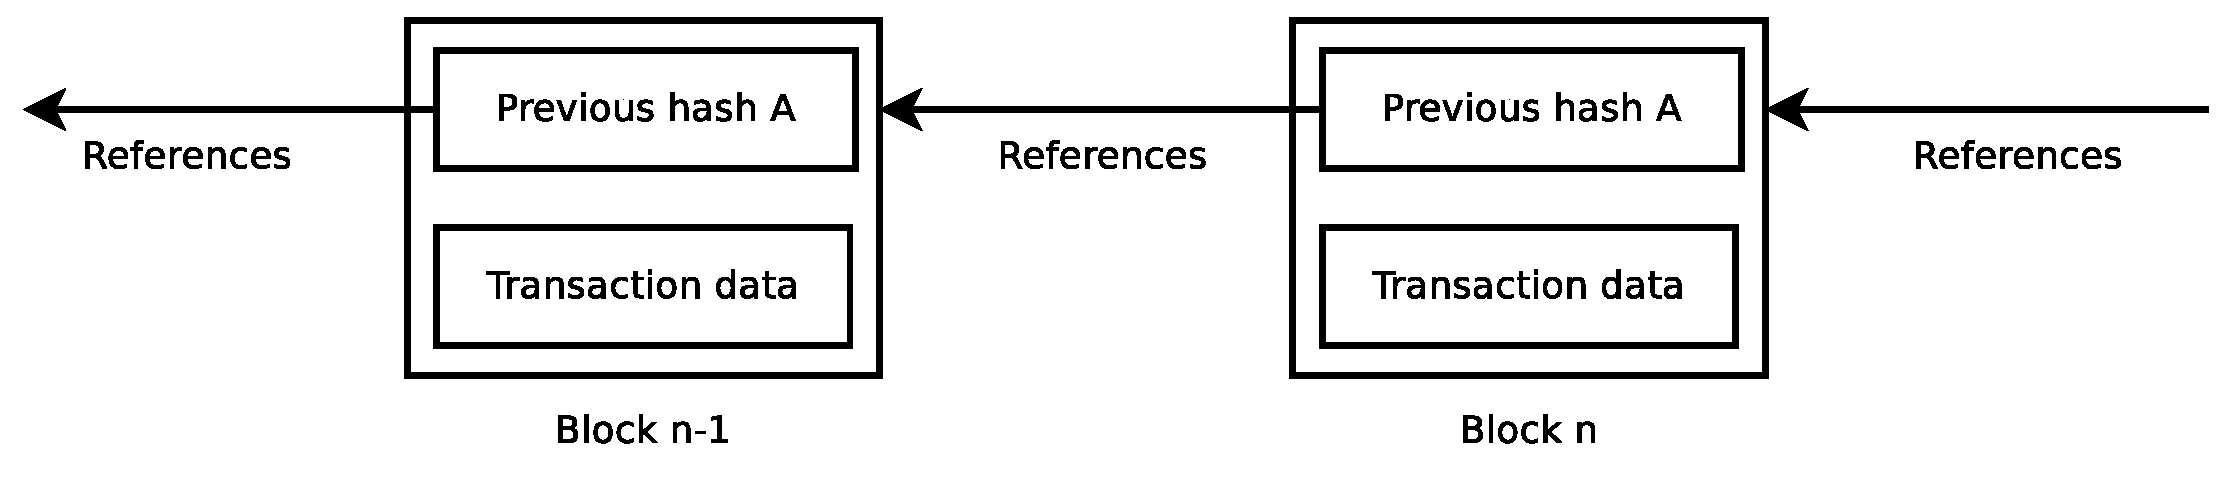
\includegraphics[scale=0.3]{design/figs/transaction-chain.eps}}
	\caption{A chain of blocks in MultiChain.}
	\label{fig:transaction-chain}
\end{figure}
